\documentclass[usenames,dvipsnames,notes,11pt,aspectratio=169]{beamer}
\usepackage{ifthen}
\usepackage{xcolor}
\usepackage{pgfplots}
\usepackage{amsmath}
\usepackage{centernot}
\usepackage{pifont}
\usepackage{tabularx}
\usepackage{makecell}
\usepackage{cuted}
\usepackage{booktabs}
\usepackage{array}
\usepackage{setspace}
\usepackage{CJKutf8}
\usepackage{textcomp}
\usepackage{subcaption}
\usepackage{inconsolata}
\usepackage{xspace}
\usepackage{pdfcomment}
%\newcommand{\pdfnote}[1]{\marginnote{\pdfcomment[icon=note]{#1}}}
\newcommand{\pdfnote}[1]{}
\newcommand\w[1]{\textit{#1}}

\pgfplotsset{compat=1.17}

\input ../beamer-style
\input ../std-macros
\input ../macros

\AtBeginSection[]
{
    \begin{frame}
        \frametitle{Table of Contents}
        \tableofcontents[currentsection]
    \end{frame}
}


\title[DS-GA.1011]{Text classification}
\author[He He]{He He
}
\institute[NYU]{
    
\includegraphics[height=1cm]{../figures/nyu-logo}\\
}
\date{September 6, 2023}

%\includeonly{conclusion}
%\includeonlyframes{current}

\begin{document}

\begin{frame}
\titlepage
\end{frame}

\section{Course overview}

\subsection{Logistics}
\begin{frame}
{Logistics}
    \begin{itemize}
        \item Instructor: He He
        \item Section leaders: Lavender Jiang, Xiang Pan, Weizhe Yuan, Yilun Kuang (see the Staff page)
        \item Graders: Lavender Jiang, Xiang Pan, Yilun Kuang, Danielle Rothermel
    \end{itemize}
    \begin{itemize}
        \item Best way to communicate with us: \textbf{Campuswire} (link and code on Brightspace).
        \item Office hours will be in-person or on Zoom (see the Staff page).
        \item Let us know if you have accessibility needs.
    \end{itemize}
\end{frame}

\begin{frame}
    {What this course is (not) about}
    \begin{itemize}
        \itemsep1em
        \item It's not about specific NLP applications (QA, dialogue etc.)
            \begin{itemize}
        \item Unified approaches to various NLP problems
        \item Hands-on experience in building NLP systems (\eg machine translation) through assignments and the course project
            \end{itemize}

            \pause
        \item It's not about fundamental machine learning and deep learning
            \begin{itemize}
        \item Focus on unique challenges in language data
        \item Formalize NLP tasks as statistical learning problems
        \item Focus on modern techniques (\eg word vectors, neural networks, large language models)
            \end{itemize}
    \end{itemize}
\end{frame}

\begin{frame}
    {What we expect you to know}
    \begin{itemize}
        \itemsep1em
        \item \textbf{Linear algebra}: vector space, vector norm, dot product, gradient etc.
        \item \textbf{Probability and statistics}: conditional probability, expectation, Bayes rule etc.
        \item \textbf{Basic machine learning}: loss function, gradient descent, logistic regression etc.
        \item \textbf{Programming}: read and write Python code, use Numpy, HPC, and deep learning libraries (Pytorch, Huggingface etc.)
    \end{itemize}
\end{frame}

\begin{frame}
    {Course project}
    An important component of the course (more on this later)
    \begin{itemize}
        \itemsep1em
        \item Related to NLP (doesn't have to be in the scope of this course)
        \item New algorithms or models for existing problems
        \item Applications of NLP or ML techniques to a problem
        \item Analysis of well-known approaches that leads to new insight
        \item ML Reproducibility Challenge 2021 (\url{https://paperswithcode.com/rc2021}) 
    \end{itemize}
\end{frame}

\subsection{A brief history of NLP/AI}
\begin{frame}
    {Products powered by NLP technologies}
    \begin{tikzpicture}
        \node (translation) {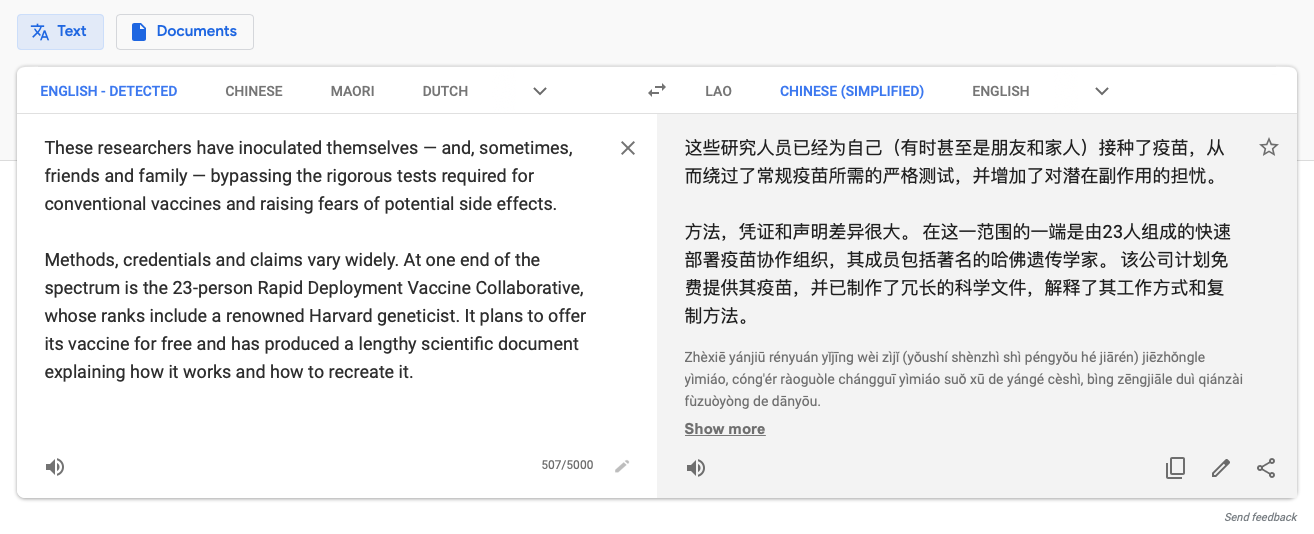
\includegraphics[width=10cm]{figures/google-translate}};
        \node (qa) [below= of translation, anchor=north east, yshift=3em]{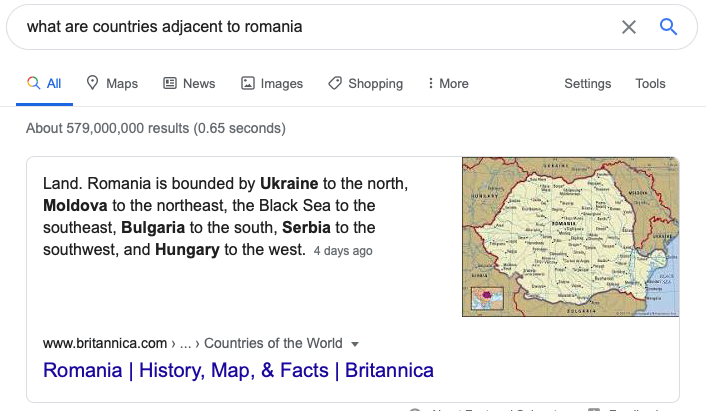
\includegraphics[width=5cm]{figures/search-qa}};
        \node [right= of qa]{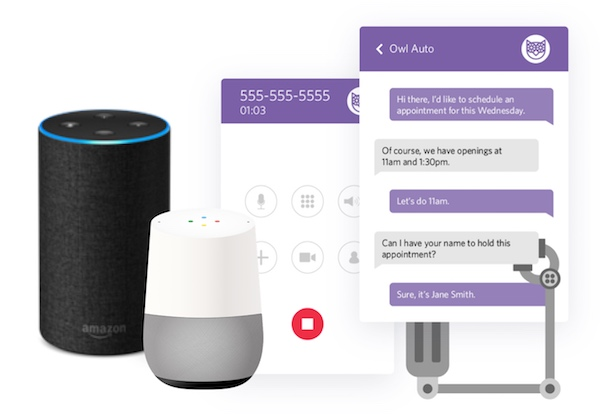
\includegraphics[width=5cm]{figures/alexa}};
    \end{tikzpicture}
\end{frame}

\begin{frame}
    {A single natural language interface for everything}
    \begin{figure}
        
\includegraphics[width=10cm]{figures/chatgpt-1}
    \end{figure}
\end{frame}

\begin{frame}
    {A single natural language interface for everything}
    \begin{figure}
        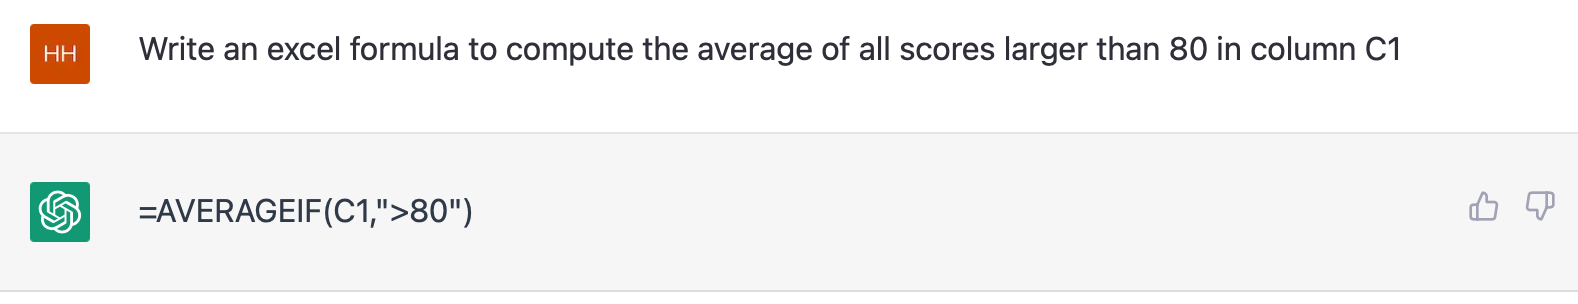
\includegraphics[width=10cm]{figures/chatgpt-2}
    \end{figure}
\end{frame}

\begin{frame}
    {Language is at the core of AI: the imitation game}
    \begin{figure}
        \begin{subfigure}[b]{0.4\textwidth}
        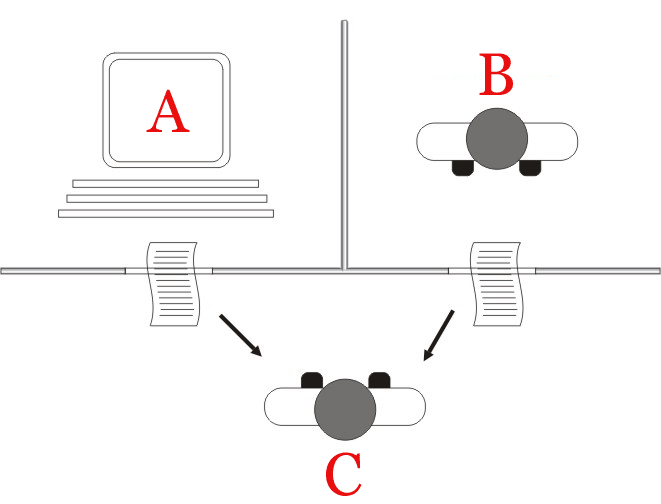
\includegraphics[height=3cm]{figures/turing-test}
        \end{subfigure}\hfill
        \begin{subfigure}[b]{0.4\textwidth}
        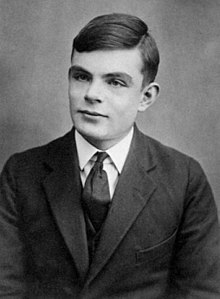
\includegraphics[height=4cm]{figures/turing}
        \end{subfigure}
    \end{figure}
    \pdfnote{The interrogator chats with two agents and must tell which is human vs AI.}

    \nl{I believe that in about \blue{fifty years'} time it will be possible to programme computers, with a \blue{storage capacity of about $10^9$}, to make them play the imitation game so well that an average interrogator will not have more than 70 percent chance of making the right identification after five minutes of questioning.} Turing (1950)
    %I believe that at the end of the century the use of words and general educated opinion will have altered so much that one will be able to speak of machines thinking without expecting to be contradicted.'' 
    \pdfnote{Alan Turing proposed the famous Turing test as a criteria for intelligence, where an interrogator tries to distinguish between a computer and a real human through text-based conversation. Turing was optimistic that a machine will pass the Turing test by the end of the century and possess human thinking capability. We are obviously far from that. But a more interesting question is, even if a machine passes the Turing test, does it mean it has acquired human intelligence?}

    \pause\medskip
    \think{Is humanlikeness the ultimate goal?}
    \pdfnote{You can have a not so smart AI which an fake humanlikeness, or a superhuman AI that can be detected by the interrogator.}
    \pdfnote{In practice, evaluating AI is a challenging task, moving goal post, test coverage etc.}
\end{frame}

\begin{frame}
    {ELIZA}
    \begin{itemize}
        \item Built by Joseph Weizenbaum at MIT in 1964 to demonstrate the \emph{superficiality} of human-machine communication.
        \item Surprisinly, people were convinced that ELIZA had human intelligence.
    \end{itemize}
    \bigskip
    \centering
    \begin{table}
        \begin{tabular}{ll}
            Human: & Well, \blue{my boyfriend made me come here}.\\
            ELIZA: & \red{Your boyfriend made you come here}?\\
            Human: & He says \blue{I'm depressed} much of the time.\\
            ELIZA: & I am sorry to hear \red{you are depressed}.\\
            Human: & It's true. I'm \blue{unhappy}.\\
            ELIZA: & Do you think coming here will help you \red{not to be unhappy}?
        \end{tabular}
    \end{table}
    \pdfnote{ELIZA was the first chat bot that was able to attempt the Turing test. Unlike the IBM-Georgetown experiment that was meant to showcase the capability of machines, Elizabuilt was built by Joseph Weizenbaum to demonstrate the superficiality of human-machine communication. The bot was able to simulate a psychotherapist using simple pattern matching, mostly just slightly rephrasing the patients’ utterance. Nevertheless, many early users were convinced that it has human intelligence.}
\end{frame}

\begin{frame}
    {Early rule-based systems: the Georgetown-IBM experiment}
    \begin{itemize}
        \item The Russian-English machine translation program:\\
            \begin{center}
            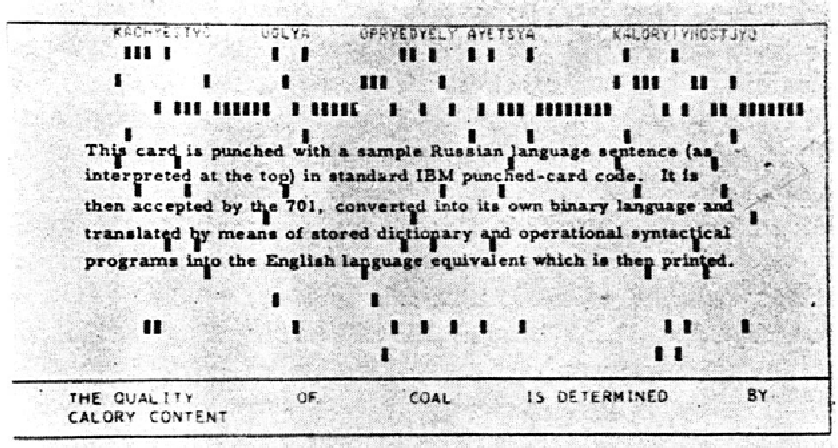
\includegraphics[height=3cm]{figures/ibm-experiment}
            \end{center}
        \item A vocabulary of \blue{250 words}
        \item Using \blue{6 grammar rules}, \eg\\
            \texttt{
                If first code is 110, is third code associated with preceding complete word equal to 21? If so, reverse order of appearance of words in output (i.e., word carrying 21 should follow that carrying 110)---otherwise, retain order.}
    \end{itemize}
    \pdfnote{Aside from the philosophical arguments, there is clear practical motivation for working on NLP. Machine translation (MT) is one such example. In fact, interests in building MT systems started even before AI. The Georgetown-IBM experiment is the first public demonstration of a MT system. It has six grammar rules and a vocabulary of size 250, and was able to translate more than 60 sentences from Russian to English. The demonstration was widely covered and encouraged subsequent funding in MT.}
\end{frame}

\begin{frame}
    {Approaching AI as a whole: SHRDLU}
    \begin{columns}
        \begin{column}{0.6\textwidth}
    \begin{itemize}
        \item Built by Terry Winograd at MIT in 1968.
        \item A person instructs the computer to build structures in a blocks world.
        \item \blue{Require many skills}: grounding, coreference resolution, question answering, semantic parsing etc. 
    \end{itemize}
        \end{column}
        \begin{column}{0.4\textwidth}
    \begin{center}
    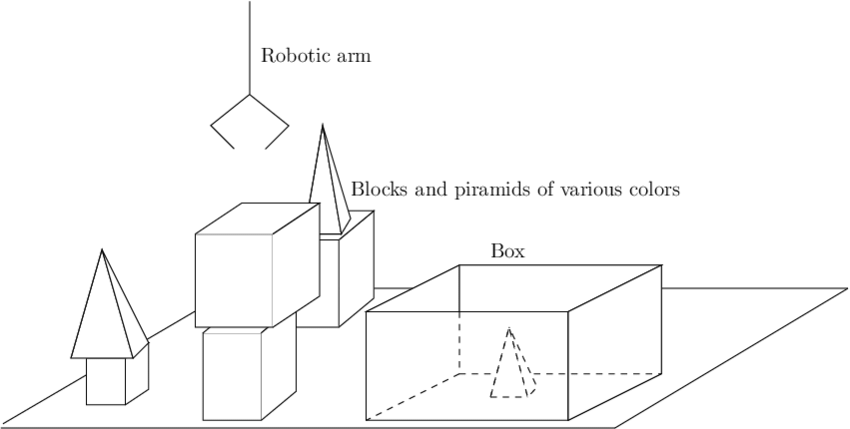
\includegraphics[height=3cm]{figures/shrdlu}
    \end{center}
        \end{column}
    \end{columns}
    \begin{table}
        \begin{tabular}{lp{12cm}}
            Person:& Pick up a big red block.\\
            Computer:& OK.\\
            Person:& Grasp the pyramid.\\
            Computer:& I don't understand which pyramid you mean.\\
            Person:& (changing their mind) Find a block which is taller than the one you are holding and put it into the box.\\
            Computer:& By "it", i assume you mean the block which is taller than the one i am holding.
    \end{tabular}
    \end{table}
    \pdfnote{Another feature of early efforts in AI is that people try to build general AI systems as opposed to domain/task specific systems.}
    \pdfnote{Terry Winograd’s SHRDLU is another successful demonstration of AI. It can interact with users in natural language and take actions in blocks world. The system demonstrated advanced language understanding skills in this simple world, e.g., grounding, question answering, semantic parsing, coreference resolution, clarification etc. Unfortunately, subsequent effort in scaling it up to more complex settings failed, which is a common weakness of earlier AI systems.}
\end{frame}

\begin{frame}
    {Limitations of early systems}
    \begin{itemize}
        \itemsep1em
        \item Optimism in the 50's and 60's: working on tasks that are too complex at that time\\[1ex]
            \nl{Within the very near future---much less than twenty-five years---we shall have the technical capability of substituting machines for any and all human functions in organizations.}
        \item Disappointing results due to
            \begin{itemize}
                \item \textbf{Limited computation}: hardware has limited speed and memory 
                \item \textbf{Combinatorial explosion}: algorithms are intractable in realistic settings
                \item \textbf{Underestimated complexity}: ambiguity, commonsense knowledge etc.
            \end{itemize}
    \end{itemize}
\end{frame}

\begin{frame}
    {The rise of statistical learning in the 80's}
    \begin{itemize}
        \itemsep1em
        \item Notable progress in MT from IBM (neglected knowlege of linguistics).
        \item HMMs widely used for speech recognition.\\
            \nl{Every time I fire a linguist, the performance of the speech recognizer goes up.}---Frederick Jelinek.
        \item The paradigm shift: \blue{expert knowledge + rules $\rightarrow$ data + features}
        \item Statistical learning is the main driving force of NLP today.
    \end{itemize}
\end{frame}

\begin{frame}
    {The deep learning tsunami}
    \begin{itemize}
        \itemsep1em
        \item Before deep learning (around 2015), NLP is mostly about structured prediction and feature engineering.
        \item Neural networks can automatically learn good features/representations for a task 
        \item The paradigm shift: \blue{features $\rightarrow$ network architectures + embeddings}
        \item Almost all NLP models are neural networks nowadays.
    \end{itemize}
\end{frame}

\begin{frame}
    {Models and data keep getting larger}
    \begin{itemize}
        \itemsep1em
        \item Since around 2018, Transformer-based pretrained models have become the standard. 
        \item Pre-training on large data provides useful representations for many downstream tasks.
        \item The paradigm shift: \blue{architecture design $\rightarrow$ transfer learning (fine-tuning)}
        \item More recently, a single natural language interface for all tasks (\eg ChatGPT by OpenAI).
        \item The paradigm shift: \blue{transfer learning $\rightarrow$ instructing / prompting}
    \end{itemize}
\end{frame}

\subsection{Challenges in NLP}

\begin{frame}
    {Why is language hard?}
    \pause
    \begin{itemize}
        \item \textbf{Discrete}
            \begin{itemize}
                \itemsep1em
                \item How to define metrics?
                    \\\medskip
                    \begin{tabular}{lcl}
                        I work \blue{at} NYU. & vs & I work \blue{for} NYU. \\
                        This is good. & vs & This is \blue{actually} good.
                    \end{tabular}
                \item How to define transformations?\\
                    \medskip
                    \begin{tabular}{p{7cm}cp{5cm}}
                    The food is okay. & $\rightarrow$ & The food is awesome! \\
                    They made a brief return to Cambridge to drop the book. & $\rightarrow$& They returned.
                    \end{tabular}
                \item In general, hard to represent text as mathematical objects.
            \end{itemize}
    \end{itemize}
    \begin{table}
    \end{table}
\end{frame}

\begin{frame}
    {Why is language hard?}
    \begin{itemize}
        \item \textbf{Compositional}
            \begin{itemize}
                \item The whole is built from parts (chars, words, sentences, paragraphs, documents...)
                \item How to generalize when we don't see all possible combinations?\\
                \item An example from \mycite{Lake et al., 2018}\\
                Vocabulary:\\
                    \begin{itemize}
                    \item[]\{jump, walk, turn, once, twice, left, right, before, after, and\}
                    \end{itemize}
                Sentences: \\
                    \begin{itemize}
                       \item[]jump \\
                       \item[]jump left\\
                       \item[]jump left and walk right \\
                       \item[]jump left after walk right once before turn left twice\\
                       \item[]...
                    \end{itemize}
            \end{itemize}
    \end{itemize}
\end{frame}

\begin{frame}
    {Why is language hard?}
    \begin{itemize}
        \item \textbf{Sparse} 
            \begin{itemize}
                \item How to handle the long tail?
                \item Zipf's law: $\text{word frequency} \propto \frac{1}{\text{rank}}$
                    \begin{figure}
                        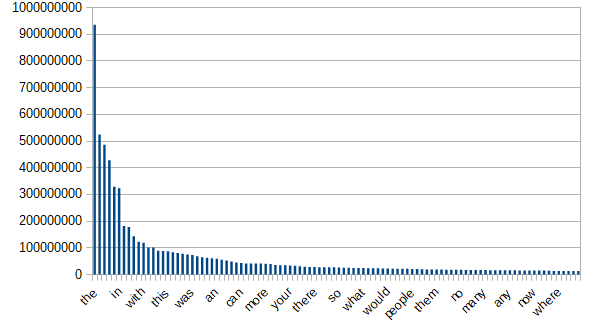
\includegraphics[height=3cm]{figures/zipf}
                    \end{figure}
                \item Many linguistic phenomena follow Zipf's law\\
                    BoA's financial assistant Erica:\\
                    \textit{The bank ``learned [that] there are over 2,000 different ways to ask us to move money.''}\footnote[frame]{
                        \url{https://www.aiqudo.com/2019/06/28/voice-success-story-erica-bank-america/}
                    }
            \end{itemize}
    \end{itemize}
\end{frame}

\begin{frame}
    {Why is language hard?}
    \begin{itemize}
        \item \textbf{Ambiguous} 
            \begin{itemize}
                \item How to interpret meaning in context?
                \medskip
                \begin{itemize}
                    \itemsep2em
                    \item[] Bass: fish? guitar? frequency? (word sense disambiguiation)
                    \item[] I shot an elephant in my pajamas: who is in the pajamas? (PP attachment)
                    \item[] The spirit is willing but the flesh is weak.\\
                        $\rightarrow$ 
                        The vodka is strong but the meat is rotten.
                \end{itemize}
            \end{itemize}
    \end{itemize}
\end{frame}

\section{Supervised learning basics}

\subsection{Generalization}
\begin{frame}
    {Rule-based approach}
\begin{figure}
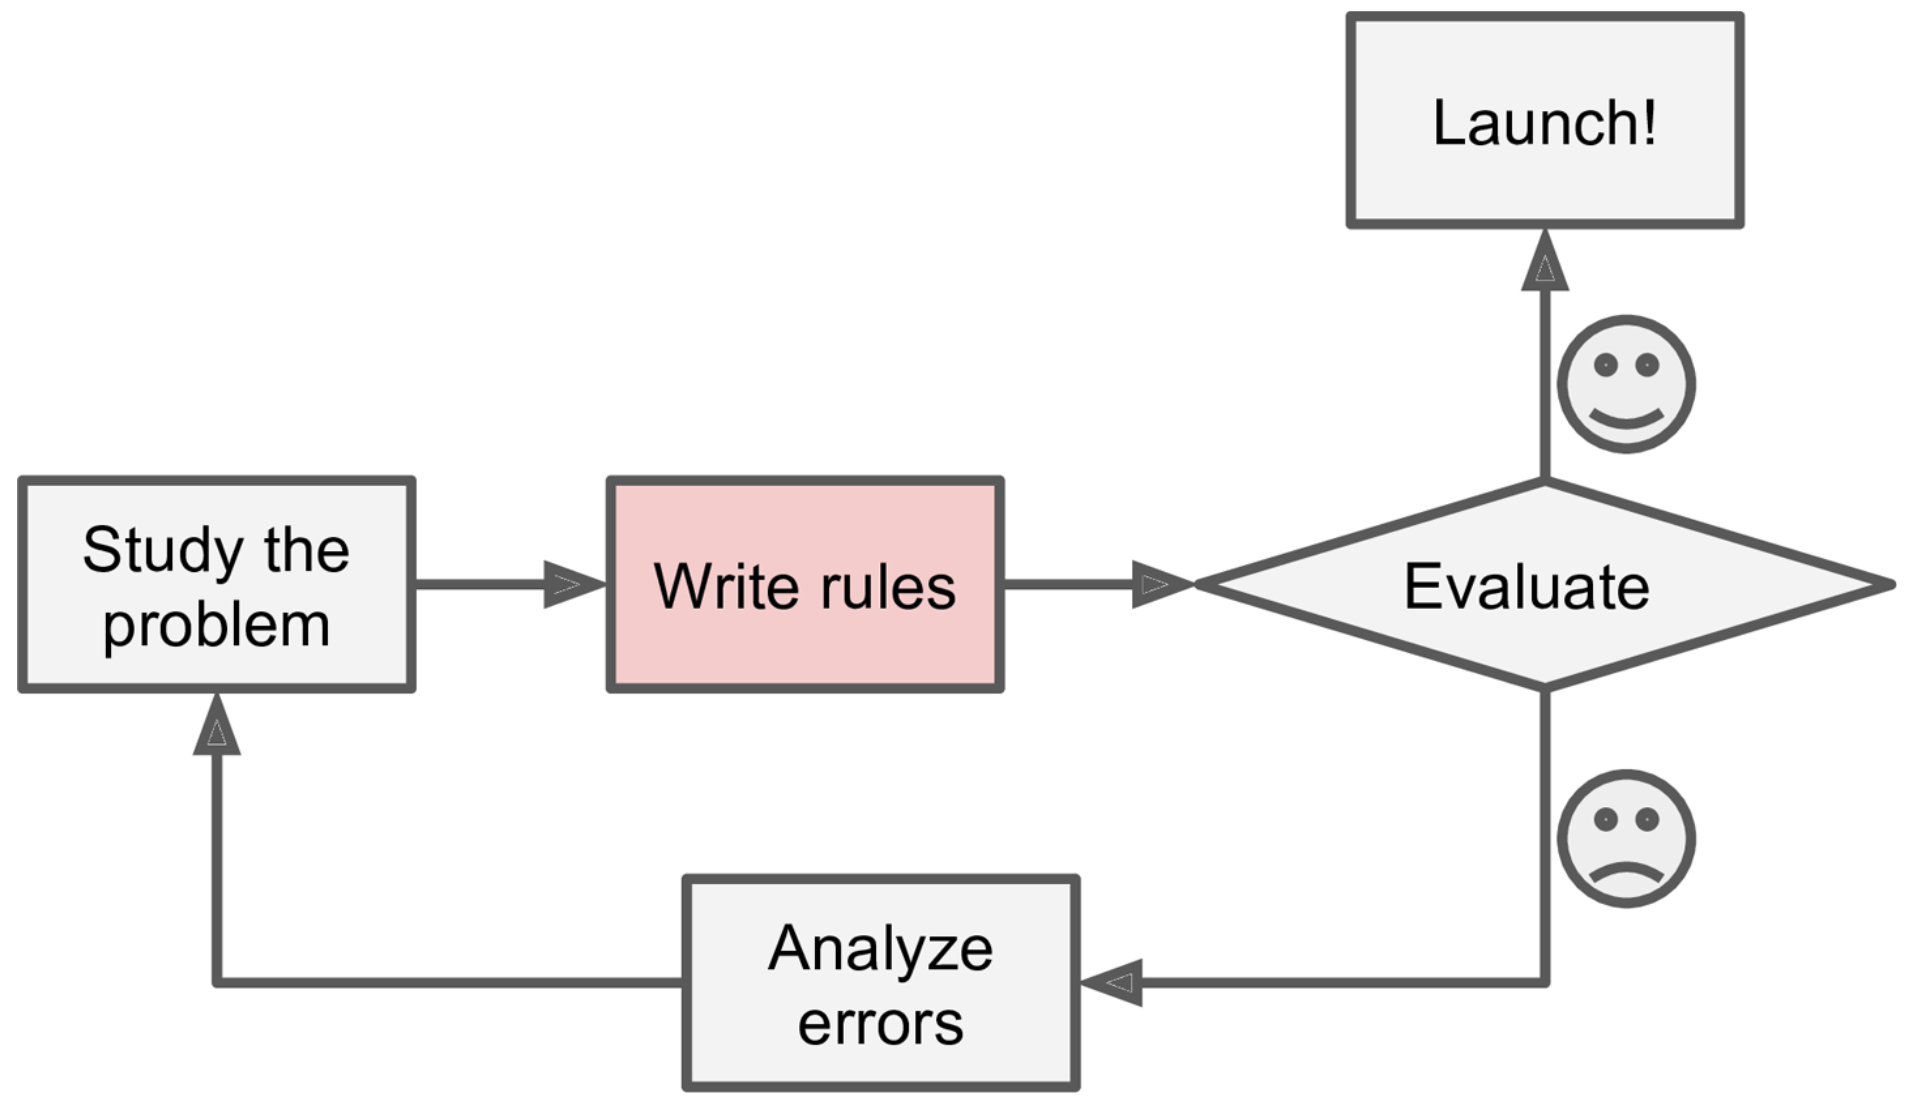
\includegraphics[height=0.7\textheight]{figures/geron-fig1-1}
    \caption{{Fig 1-1 from \emph{Hands-On Machine Learning with Scikit-Learn and TensorFlow} by Aurelien Geron (2017).}}
\end{figure}
\end{frame}

\begin{frame}
    {Machine learning approach}
\begin{figure}
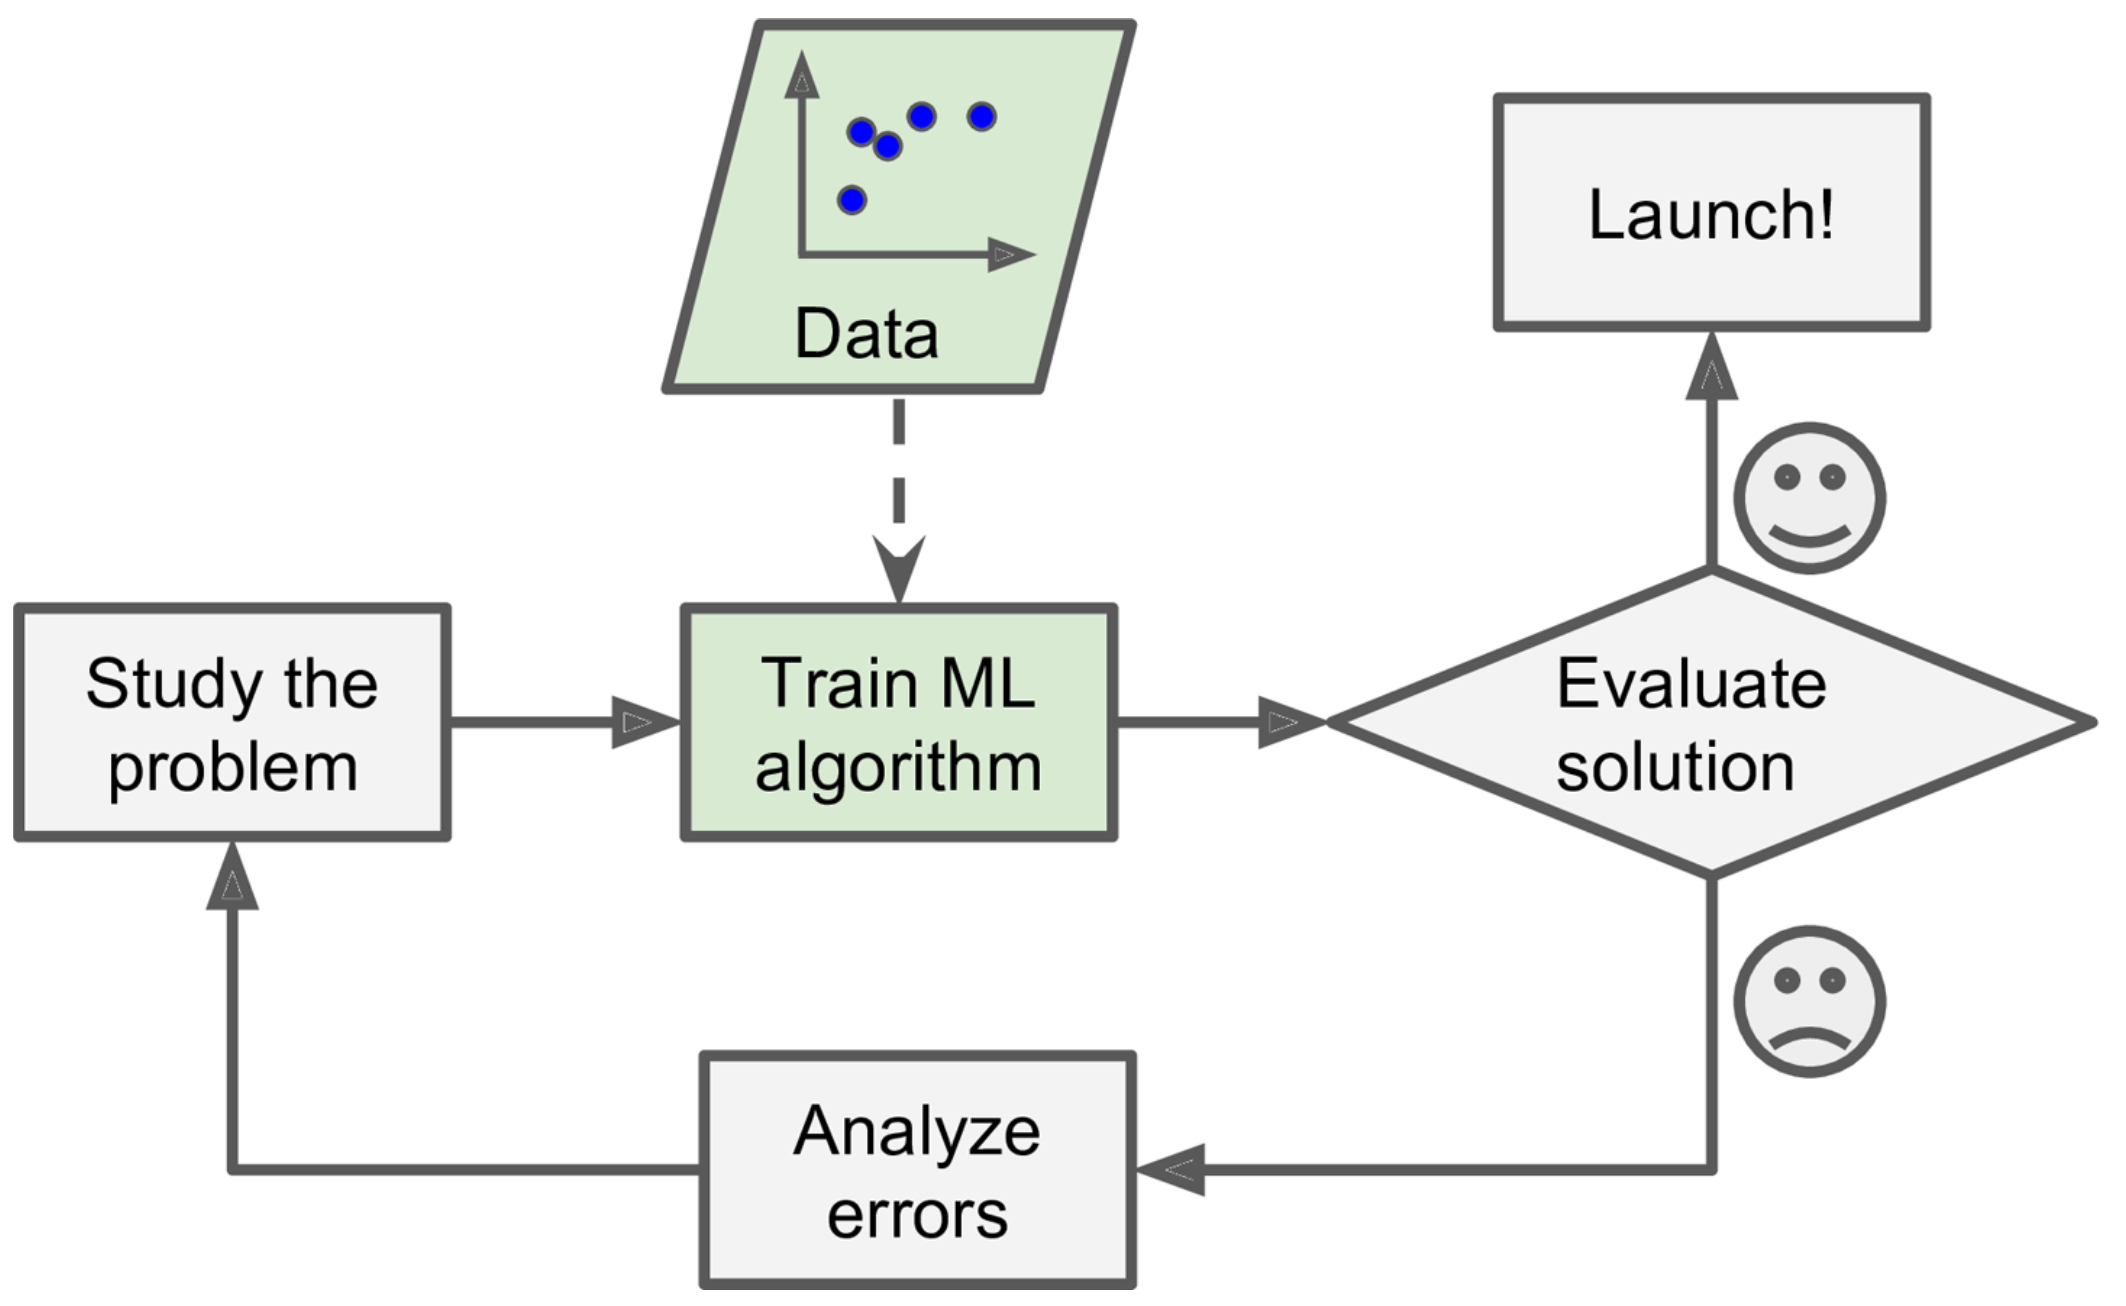
\includegraphics[height=0.7\textheight]{figures/geron-fig1-2}
    \caption{{Fig 1-2 from \emph{Hands-On Machine Learning with Scikit-Learn and TensorFlow} by Aurelien Geron (2017).}}
\end{figure}
\end{frame}

\begin{frame}
    {Example: spam filter}
    
    \begin{itemize}
        \itemsep1em
        \item Rules
            \begin{itemize}
                \item[] Contains ``Viagra''
                \item[] Contains ``Rolex''
                \item[] Subject line is all caps
                \item[] ... 
            \end{itemize}
        \item Learning from data
            \begin{enumerate}
                \item Collect emails labeled as spam or non-spam 
                \item Design features, e.g., first word of the subject, nouns in the main text
                \item Learn a binary classifier 
            \end{enumerate}
    \end{itemize}
    \medskip\pause
    \think{Pros and cons of each approach?}
\end{frame}

\begin{frame}
    {Key challenges in machine learning}
    \begin{itemize}
        \itemsep1em
        \item Availability of large amounts of (annotated) data
            \begin{itemize}
                \item Data collection: scraping, crowdsourcing, expert annotation
                \item Quality control: data quality can have large impact on the final model (garbage in garbage out)
                \item Don't take it for granted: always check the data source!
            \end{itemize}
    \end{itemize}
    \medskip\pause
    \think{How would you collect a dataset for the spam filtering task?}
\end{frame}

\begin{frame}
    {Key challenges in machine learning}
    \begin{itemize}
        \item \textbf{Generalize} to unseen samples
            \begin{itemize}
                \item We want to build a model: $h\colon \sX \text{ (input space)} \rightarrow \sY \text{ (output space)}$
                \item It is easy to achieve high accuracy on the training set.
                \item But we want the model to perform well on unseen data, too.
                \item What should be the learning objective? 
               %\item Given the training set: $m$ samples from $\sD$ $\pc{(x^{(i)}, y^{(i)})}_{i=1}^m$
               % \item Assume that there is a (unknown) data generating distribution: $\sD$ over $\sX\times\sY$
               %\item Goal: \blue{minimize }:$\text{minimize}\quad 
               %    \mathbb{E}_{(x,y)\sim\sD}\pb{\text{error}(h,x,y)}$ (estimated on the test set)
            \end{itemize}
    \end{itemize}
\end{frame}

\begin{frame}
    {Empirical risk minimization (ERM)}

    \begin{itemize}[<+->]
        \item Assume a data generating distribution $\sD$ over $\sX\times\sY$ (e.g., spam writers and non-spam writers)
        \item We have access to a training set: $m$ samples from $\sD$ $\pc{(x^{(i)}, y^{(i)})}_{i=1}^m$
        \item We can measure the goodness of a prediction $h(x)$ by comparing it against the groundtruth $y$ using some \textbf{loss function}
        \item Our goal is to minimize the \blue{expected loss} over $\sD$ (\textbf{risk}):
            $$
\text{minimize}\quad \mathbb{E}_{(x,y)\sim\sD}\pb{\mathrm{error}(h,x,y)} \;,
            $$
            but it \red{cannot be computed} (why?).
\item Instead, we minimize the \blue{average loss on the training set} (\textbf{empirical risk})  %over $\sH$
    $$
    \text{minimize}\quad \frac{1}{m}\sum_{i=1}^m \mathrm{error}(h, x^{(i)}, y^{(i)})
    $$

%\item In the limit of infinite samples, empirical risk converges to risk (LLN).
\item {\bf Key question}: does small empirical risk imply small risk? 
    \end{itemize}
\end{frame}

%\begin{frame}
%    {Error decomposition}
%\end{frame}

\begin{frame}
    {Overfitting vs underfitting}
    \begin{itemize}
        \item Trivial solution to (unconstrained) ERM: \red{memorize} the data points
        \item Need to extrapolate information from one part of the input space to unobserved parts!
        \item Solution: constrain the prediction function to a subset, i.e.\ a \textbf{hypothesis space} $h\in \sH$.
            \pause
        \item Trade-off between complexity of $\sH$ and generalization 
        \item Question for us: \blue{how to choose a good $\sH$ for certain domains}
    \end{itemize}
\end{frame}

\begin{frame}
    {Summary}
    \begin{enumerate}
        \itemsep2em
        \item Obtain training data $D_{\text{train}}=\pc{(x^{(i)}, y^{(i)})}_{i=1}^n$.
        \item Choose a loss function $L$ and a hypothesis class $\sH$ (\blue{domain knowledge}).
        \item Learn a predictor by minimizing the empirical risk (\blue{optimization}).
    \end{enumerate}
\end{frame}

\subsection{Loss functions}

\begin{frame}
    {Setup}
    \begin{itemize}
        \itemsep1em
        \item Task: binary classification $y\in\pc{+1, -1}$
        \item Model: $f_w\colon \sX \rightarrow \bR$ parametrized by $w \in \bR^d$
            \begin{itemize}
                \item Output a score for each example
            \end{itemize}
        \item Prediction: $\text{sign}(f_w(x))$
            \begin{itemize}
                \item Positive scores are mapped to the positive class 
            \end{itemize}
        \item Loss functions: quantify the goodness of the model output $f_w(x)$ given $y$
    \end{itemize}
\end{frame}

\begin{frame}
    {Zero-one loss}
    
    First idea: check if the prediction is the same as the label
    \vspace{-1em}
            \begin{align}
                L(x, y, f_w) = \1\pb{\text{sign}(f_w(x)) = y} 
                = \1\pb{\underbrace{yf_w(x)}_{\textstyle\text{margin}}\le 0}
                %= \1\pb{{yf_w(x)} \le 0}
            \end{align}
    \begin{figure}
        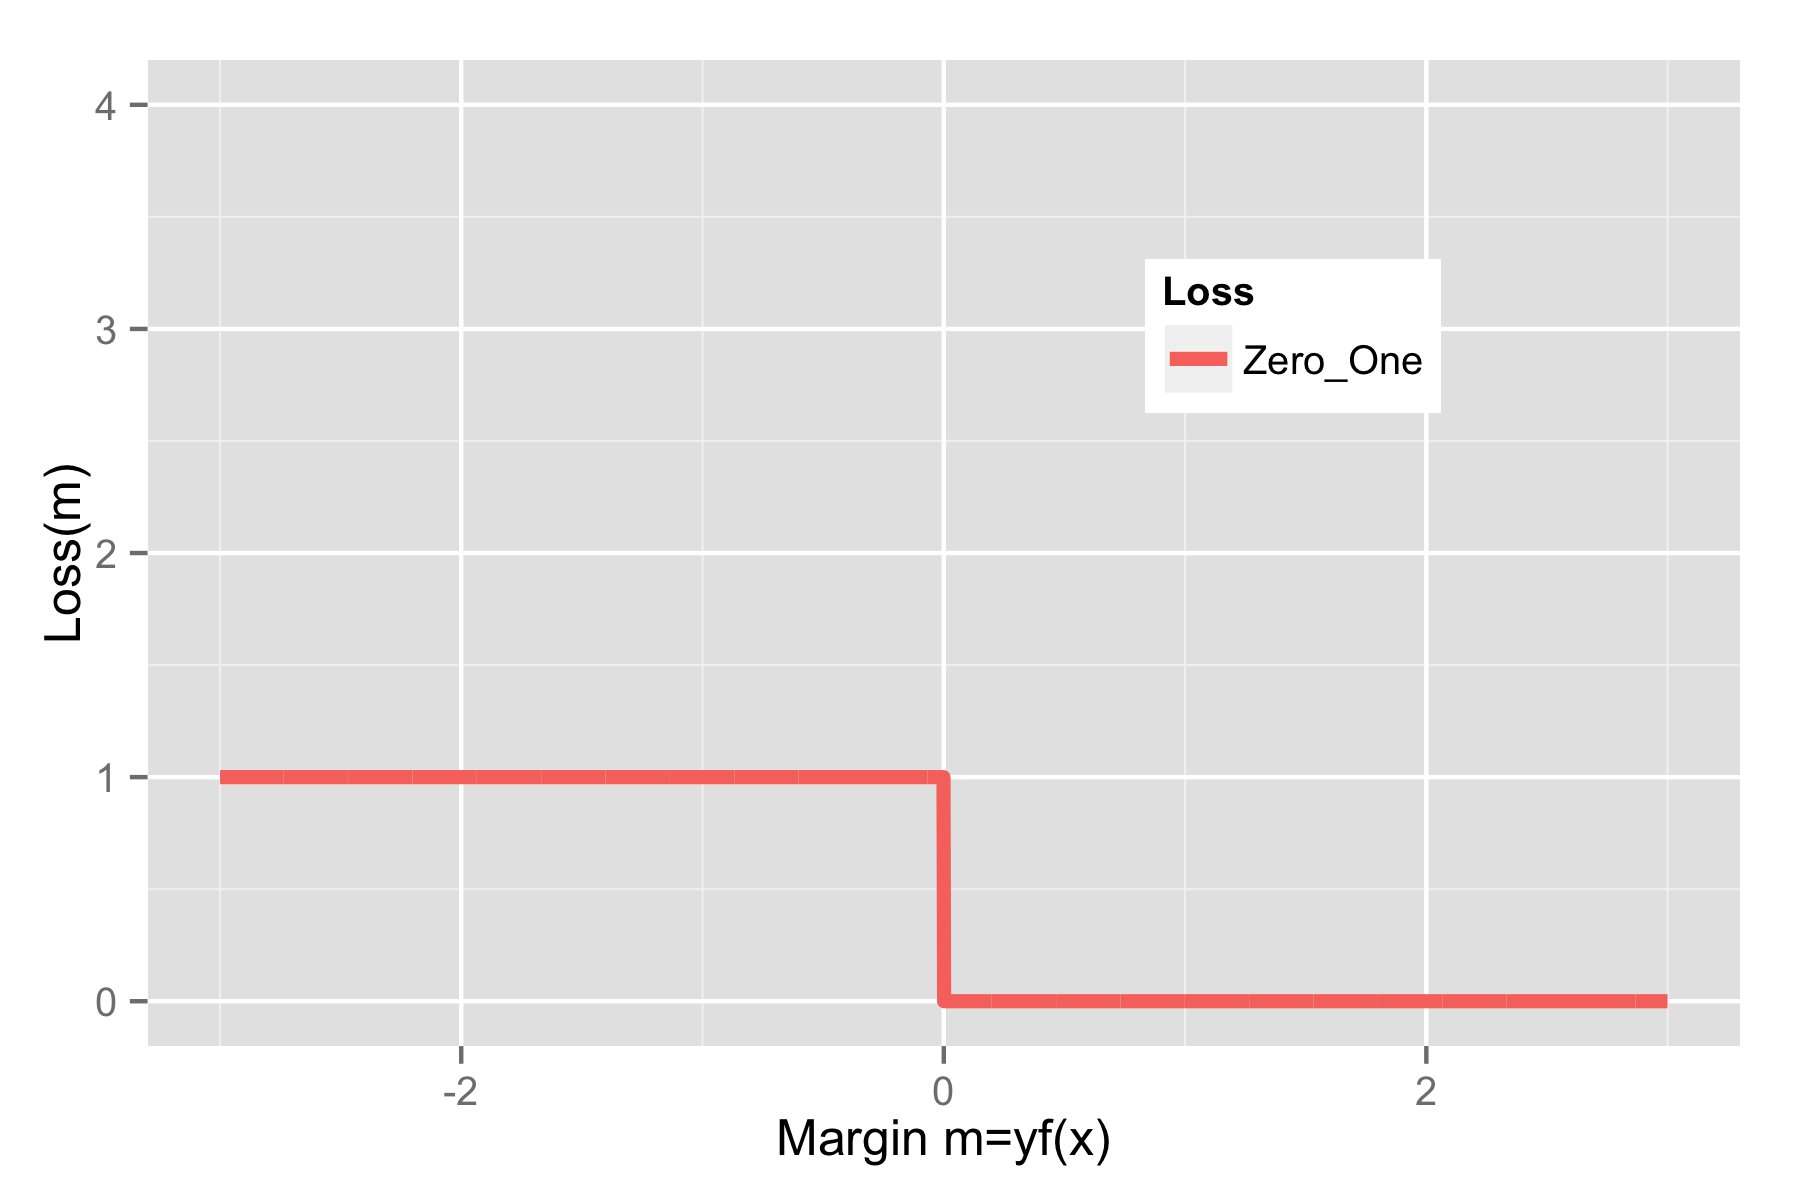
\includegraphics[height=4cm]{figures/loss.Zero_One.png}
    \end{figure}
    \pause
    Problem: \red{not differentiable}
\end{frame}

\begin{frame}
    {Hinge loss}
    $$
    L(x,y,f_w) = \max(1-yf_w(x), 0)
    $$
    \begin{figure}
        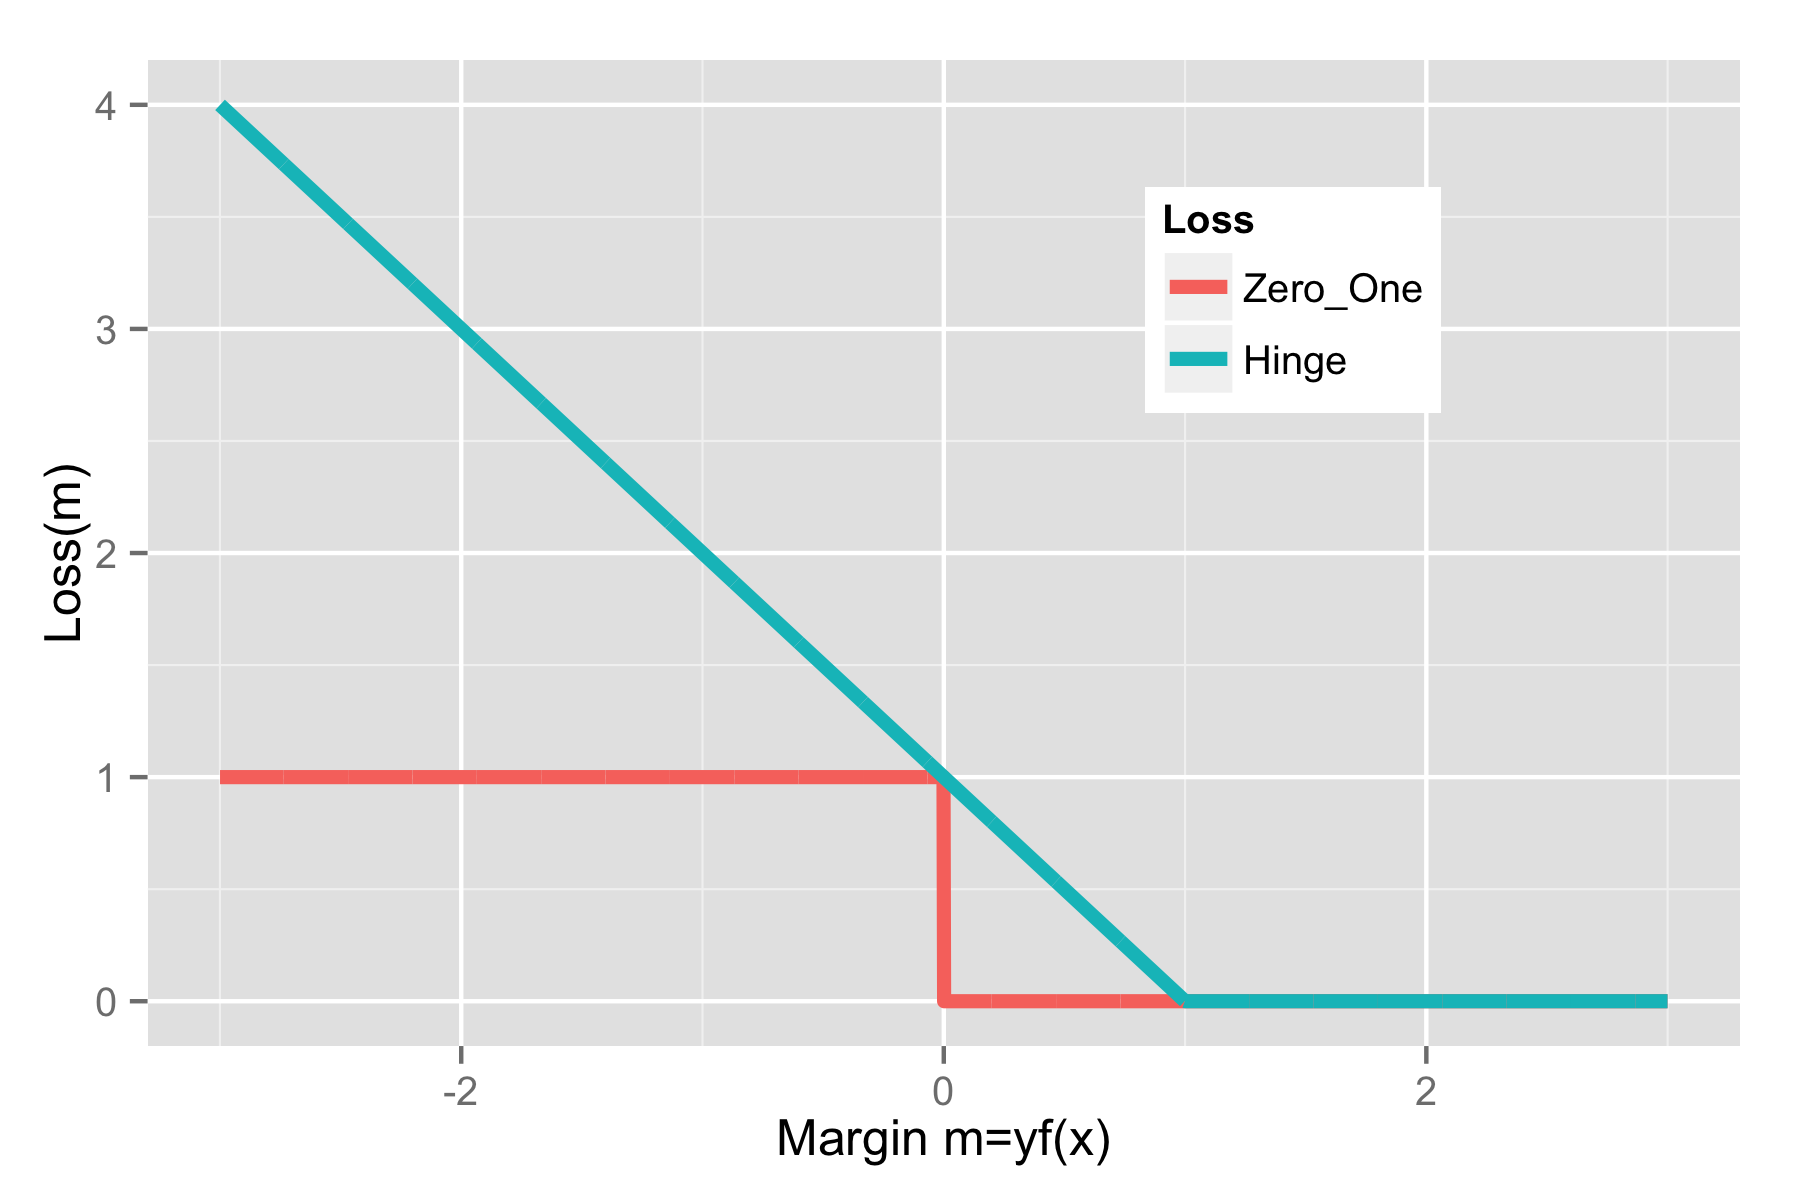
\includegraphics[height=4cm]{figures/loss.Zero_One.Hinge.png}
    \end{figure}
    \begin{itemize}
        \item A (sub)differentiable upperbound of the zero-one loss
        \item Not differentiable at $\text{margin}=1$ (use subgradients)
        %\item Subgradient: $\pc{g\colon f(x) \ge x_0 + g^T(x-x_0)}$
    \end{itemize}
\end{frame}

\begin{frame}
    {Logistic loss}
    $$
    L(x,y,f_w) = \log(1+e^{-yf_w(x)})
    $$
    \begin{figure}
        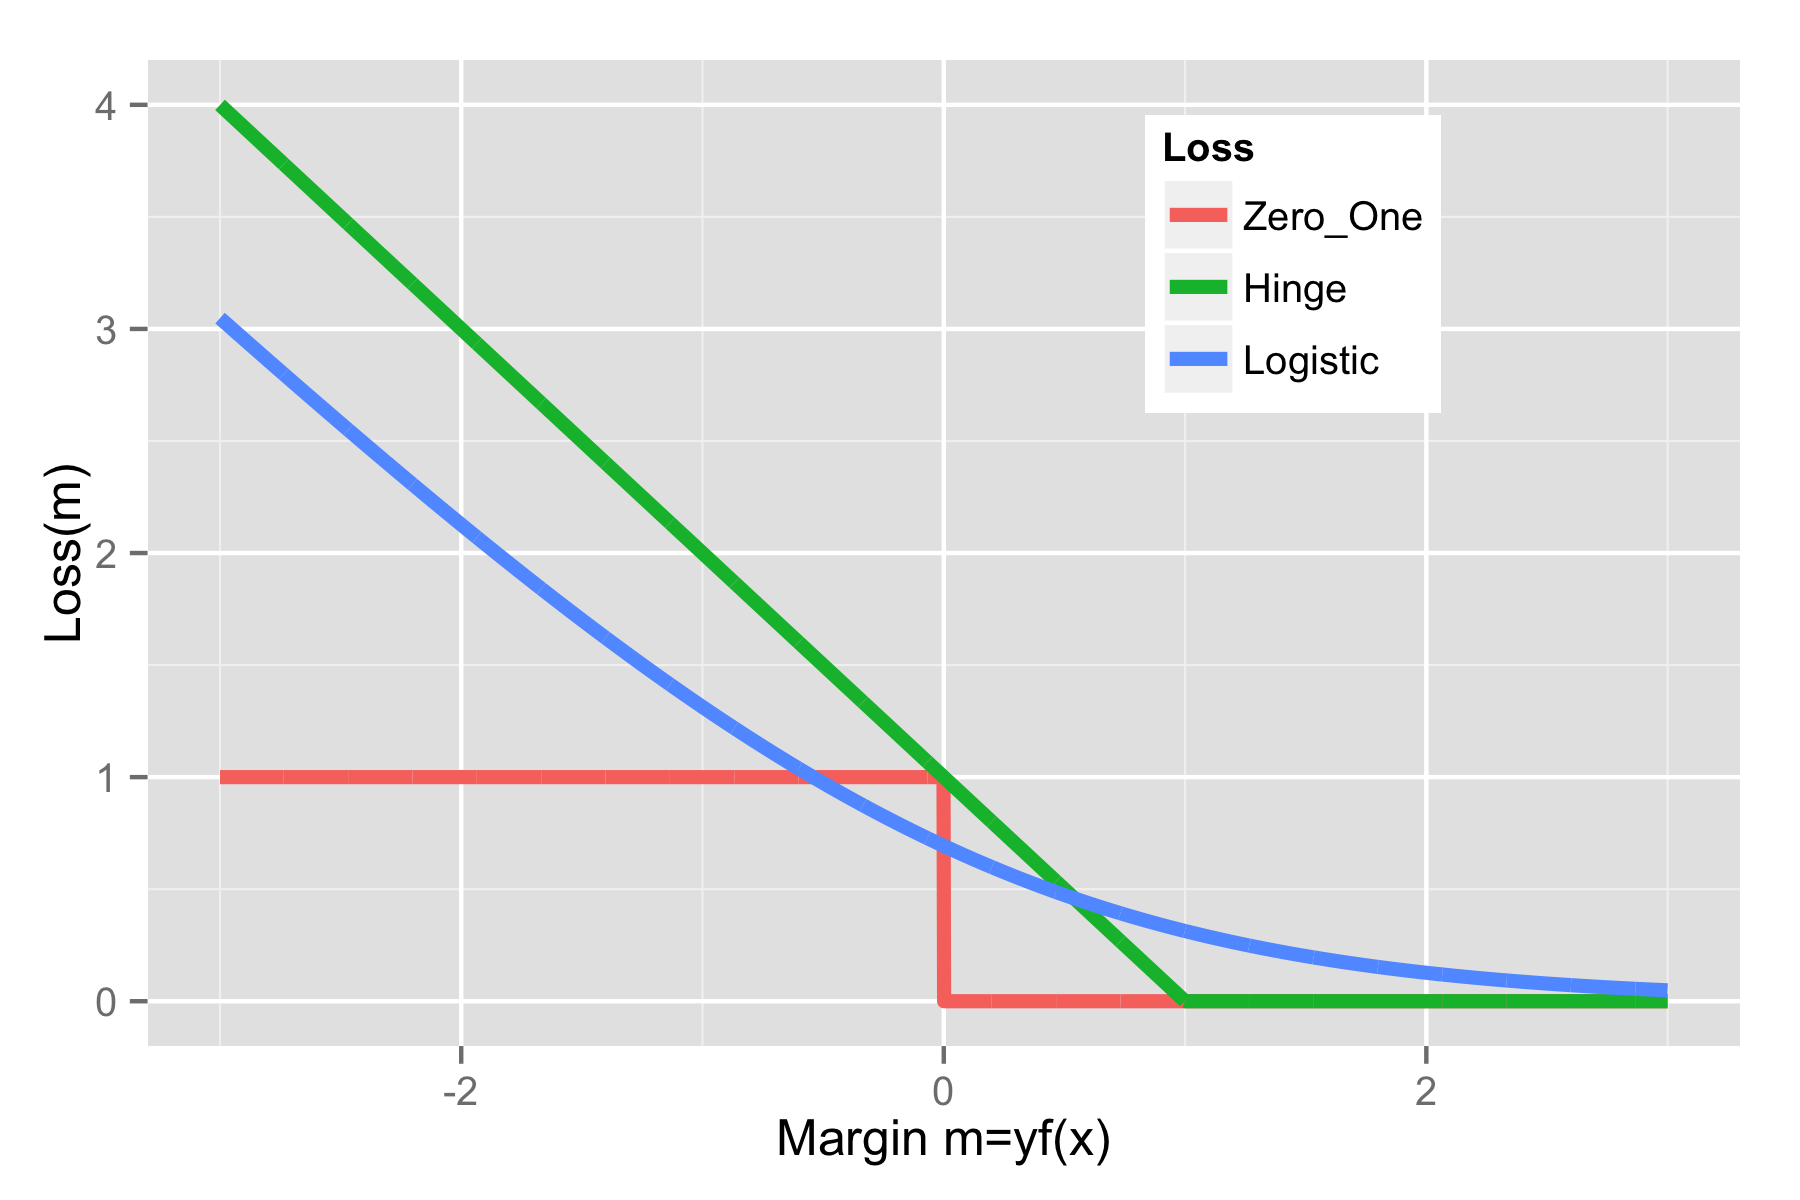
\includegraphics[height=4cm]{figures/loss.Zero_One.Hinge.Logistic.png}
    \end{figure}
    \begin{itemize}
        \item Differentiable
        \item Always wants more margin (loss is never 0)
    \end{itemize}
\end{frame}

\begin{frame}
    {Summary}
    \begin{enumerate}
        \itemsep2em
        \item Obtain training data $D_{\text{train}}=\pc{(x^{(i)}, y^{(i)})}_{i=1}^n$.
        \item Choose a loss function $L$ and a hypothesis class $\sH$ (\blue{domain knowledge}).
        \item Learn a predictor by minimizing the empirical risk (\blue{optimization}).
    \end{enumerate}
\end{frame}


\subsection{Optimization}

\begin{frame}
    {Gradient descent}
    \begin{itemize}
        \item The gradient of a function $F$ at a point $w \in \BR^d$ is the direction of fastest increase in the function value
        \item To minimze $F(w)$, move in the opposite direction
        $$w \leftarrow w - \eta\nabla_w F(w)$$
        \item Converge to a local minimum (also global minimum if $F(w)$ is \textbf{convex}) with carefully chosen step sizes $\eta$
    \end{itemize}
\end{frame}

\begin{frame}
    {Stochastic gradient descent}
    \begin{itemize}
        \item \textbf{Gradient descent (GD)} for ERM
            $$
            w \leftarrow w - \eta\nabla_w \underbrace{\sum_{i=1}^n L(x^{(i)}, y^{(i)}, w)}_{\textstyle{\text{training set loss}}}
            $$
            \pause
        \item \textbf{Stochastic gradient descent (SGD)}: take \blue{noisy but faster} updates\\
            \begin{align*}
                \text{For each } &(x, y) \in D_{\text{train}}:\\
                &w \leftarrow w - \eta\nabla_w \underbrace{L(x, y, f_w)}_{\textstyle{\text{example loss}}}
            \end{align*}
    \end{itemize}
\end{frame}

\begin{frame}
    {GD vs SGD}
    \begin{figure}
        \caption{Minimize $1.25(x + 6)^2 + (y - 8)^2$. Example from ``Understanding Machine Learning: From Theory to Algorithms''}
        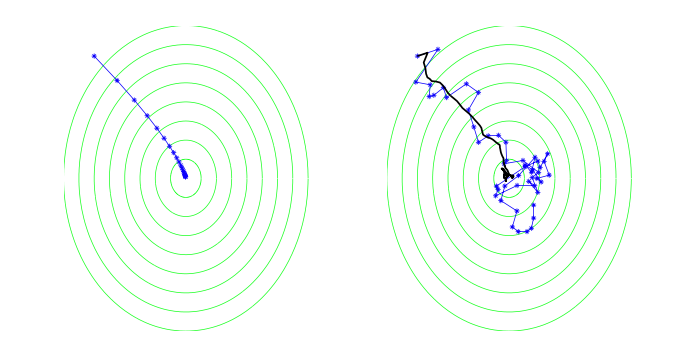
\includegraphics[height=5cm]{figures/gd-vs-sgd}
    \end{figure}
    SGD step is noisier as it gets closer to the optimum; need to reduce step size gradually.
\end{frame}

\begin{frame}
    {SGD summary}
    \begin{itemize}
        \itemsep1em
        \item Each update is efficient in both time and space
        \item Can be slow to converge 
        \item Popular in large-scale ML, including non-convex problems
        \item In practice, 
            \begin{itemize}
                \item Randomly sample examples.
                \item Fixed or diminishing step sizes, e.g. $1/t$, $1/\sqrt{t}$.
                \item Stop when objective does not improve.
            \end{itemize}
        \item Our main optimization techinque
    \end{itemize}
\end{frame}

\begin{frame}
    {Summary}
    \begin{itemize}
        \itemsep2em
        \item Choose hypothesis class based on domain knowledge
        \item Learning algorithm: empirical risk minimization
        \item Optimization: stochastic gradient descent
    \end{itemize}
\end{frame}

\section{Text classification}

\begin{frame}
    {Text classification}
    \begin{itemize}
        \item Input: text (sentence, paragraph, document)
        \item Predict the \blue{category or property} of the input text
            \begin{itemize}
                \item Sentiment classification: Is the review positive or negative?
                \item Spam detection: Is the email/message spam or not?
                \item Hate speech detection: Is the tweet/post toxic or not?
                \item Stance classification: Is the opinion liberal or conservative?
            \end{itemize}
            \pause
        \item Predict the \blue{relation} of two pieces of text
            \begin{itemize}
                \item Textual entailment (HW1): does the premise entail the hypothesis?\\
                    Premise: The dogs are running in the park.\\
                    Hypothesis: There are dogs in the park.
                \item Paraphrase detection: are the two sentences paraphrases?\\
                    Sentence 1: The dogs are in the park.\\
                    Sentence 2: There are dogs in the park.
            \end{itemize}
    \end{itemize}
    \pdfnote{
        Paraphrase detection itself may not always be a well-defined problem.
        Consider the given example, are they paraphrase?
        Well, it depends on the context.
        If the task is image caption, then yes.
        If the task is dialogue response generation, where the context is ``Where are the dogs?'',
        then S1 and S2 convey very different answers to the question.
    }
\end{frame}

\subsection{Generative models: naive Bayes}

\begin{frame}
    {Intuition}
    \begin{itemize}
        \itemsep1em
        \item \textbf{Example}: sentiment classification for movie reviews
    \begin{itemize}
        \item[] {\small \setstretch{0.8} \textit{Action. Comedy. Suspense. This movie has it
all. The Plot goes that 4 would be
professional thieves are invited to take part in a
heist in a small town in Montana. every type of
crime movie archetype character is here. Frank,
the master mind. Carlos, the weapons expert. Max,
the explosives expert. Nick, the safe cracker and
Ray, the car man. Our 4 characters meet up at the train station
and from the beginning none of them like or trust
one another. Added to the mix is the fact that
Frank is gone and they are not sure why they have
called together. Now Frank is being
taken back to New Jersey by the 2 detectives but
soon escapes on foot and tries to make his way
back to the guys who are having all sorts of
            problems of their own. \textcolor<2->{blue}{Truly a great
film loaded with laughs and great acting. Just an
overall good movie for anyone looking for a laugh
            or something a little different}}\par}
    \end{itemize}
    \pause
\item \textbf{Idea}: count the number of positive/negative words
    \pause
    \begin{itemize}
        \item What is a ``word''?
        \item How do we know which are positive/negative?
    \end{itemize}

    \end{itemize}
    \pdfnote{
        How would you quickly tell the sentiment of this review?
        Understand everything said in it is hard (genre, plot, actor performance etc.).
        But sometimes a couple of keywords or a concluding sentence is sufficient.
    }
    \pdfnote{
        Now there are two questions left.
        We know what's a word intuitively, but to the computer the input is just a string of unicodes, how can we separate that into a list of words.
        The second question is how can we tell which words are positive or negative. The rule based approach is to construct a dictionary of such words, which can be quite effective.
        But here we'll see how to learn this from labeled data.
    }
\end{frame}

\begin{frame}
    {Preprocessing: tokenization}
    \textbf{Goal}: Splitting a string of characters to a sequence of \textbf{tokens} $[x_1, \ldots, x_n]$.

    \medskip
    \textbf{Language-specific solutions}\\
    \begin{itemize}
        \itemsep1em
        \item Regular expression: ``I didn't watch the movie''. $\rightarrow$ [``I'', ``did'', ``n't'', ``watch'', ``the'', ``movie'', ``.''] 
            \begin{itemize}
                \item Special cases: U.S., Ph.D. etc.
            \end{itemize}
        \item Dictionary / sequence labeler: 
            \begin{CJK*}{UTF8}{gbsn}
                ``我没有去看电影。'' $\rightarrow$ [``我'', ``没有'', ``去'', ``看'', ``电影'', ``。'']
            \end{CJK*}
    \end{itemize}

    \medskip
    \pause
    \textbf{General solutions}: don't split by words\\
    \begin{itemize}
        \item Characters:
            [``u'', ``n'', ``a'', ``f'', ``f'', ``a'', ``b'', ``l'', ``e''] 
        \item Subword (\eg byte pair encoding):
            [``un'', ``aff'', ``able\#'']
    \end{itemize}
    \pdfnote{
        Note that for contractions like didn't. We can tokenize it into either did n't or didn 't. Both are okay as long as it's consistent.
        English tokenization gets more complex when there is punctuations or special symbols.
    }
    \pdfnote{Tokenization can have important impact on the performance of downstream learning algorithms.
    }
    \pdfnote{
        Using character sequences (or even byte sequences) we impose mininal prior knowledge on what is a word. Given enough data, the model can probably figure out a reasonable unit of the characters based on their frequencies. But one downside in this approach is that the sequence is now much longer, and the computation time of many algorithms grows with sequence length, which will be expensive for large-scale training.
    }
    \pdfnote{
        A middle ground is to use subword, a unit larger than characters but smaller than words.
        This is commonly used in large-scale models nowadays.
        The BPE algorithms is a simple technique from data compression.
        The basic idea is to recursively merge frequently adjacent symbols into a new symbol (or token).
        The subword found through this algorithm often corresponds to morphemes.
    }
\end{frame}

\begin{frame}
    {Classification: problem formulation}
    \begin{itemize}
        \itemsep1em
        \item \textbf{Input}: a sequence of tokens $x=(x_1, \ldots x_n)$ where $x_i \in \mathcal{V}$.
            \pdfnote{After tokenization, our input is no longer a seq of bytes, but a seq of tokens.}
        \item \textbf{Output}: binary label $y\in \pc{0, 1}$.
        \item \textbf{Probabilistic model}:
            $$
            f(x) = \begin{cases}
 1 & \text{if $p_\theta(y=1\mid x) > 0.5$} \\
 0 & \text{otherwise}
 \end{cases} ,
            $$
            where $p_\theta$ is a distribution parametrized by $\theta\in{\Theta}$.
        \item Modeling question: what's the parametric form of $p_\theta$?
    \end{itemize}
    \pdfnote{
        Choosing $p_\theta$ is the modeling part where our task-specific knowledge comes in: how should the label depend on the text.
    }
\end{frame}

\begin{frame}
    {Modeling $p(y\mid x)$}
    How to write a review:\\
    \pdfnote{A useful starting place for modeling is to gain some intuition on how the task is performed by humans, and then tranform that into mathematical language.}
    \begin{enumerate}
        \item Decide the sentiment by flipping a coin: $p(y)$
        \item Generate word sequentially conditioned on the sentiment  $p(x\mid y)$
    \end{enumerate}
    \pause
    \vspace{-1ex}
    \onslide<+->{
        \begin{align}
            p(y)&=\onslide<+->{\text{Bernoulli}(\alpha)} \\
            p(x\mid y)&=\onslide<+->{\prod_{i=1}^n p(x_i\mid y)\quad\quad \text{(independent assumption)}}\\
                &=\onslide<+->{\prod_{i=1}^n \text{Categorical}(
                \underbrace{\theta_{1,y},\ldots,\theta_{|\sV|,y}}_{\text{sum to 1}}
                )}
        \end{align}
    }
    \vspace{-1ex}
    \onslide<+->{
        \textbf{Bayes rule}: 
        $$
        p(y\mid x) = \frac{p(x\mid y)p(y)}{p(x)}
        = \frac{p(x\mid y)p(y)}{\sum_{y\in\mathcal{Y}} p(x\mid y)p(y)}
        $$
}
\end{frame}

\begin{frame}
    {Naive Bayes models}
    \begin{block}
    {Naive Bayes assumption}
        The input features are \textbf{conditionally independent} given the label:
        $$
        p(x\mid y) = \prod_{i=1}^n p(x_i\mid y) \;.
        $$
    \end{block}
    \begin{itemize}
        \item A strong assumption, but works surprisingly well in practice.

        \item Note: $p(x_i\mid y)$ doesn't have to be a categorical distribution (\eg Gaussian distribution)
    \end{itemize}

\end{frame}

\begin{frame}
    {Learning: maximum likelihood estimation}
    \textbf{Task}: estimate parameters $\theta$ of a distribution $p(y; \theta)$ given i.i.d. samples $D=\p{y_1, \ldots, y_N}$ from the distribution.

    \medskip
    \textbf{Goal}: find the parameters that make the observed data most probable.

    \medskip\pause
    \textbf{Likelihood function} of $\theta$ given $D$:
    $$
    L(\theta; D) \eqdef p(D;\theta) = \prod_{i=1}^N p(y_i; \theta) \;.
    $$

    \textbf{Maximum (log-)likelihood estimator}:
    \begin{align}
        \hat{\theta} &= \argmax_{\theta\in\Theta} L(\theta; D)
        = \argmax_{\theta\in\Theta} \sum_{i=1}^N \log p(y_i; \theta)
    \end{align}

    \pdfnote{To make ``most probable'' more precise, we define the likelihood function of the parameters to be the probability of the data given by the model.}
    \pdfnote{Why can we write the joint distribution as the product? Independent assumption from iid.}
    \pdfnote{Now it's reduced to an optimization problem.}
\end{frame}

\begin{frame}
    {MLE and ERM}
    ERM:
    $$
    \min \sum_{i=1}^N \ell(x^{(i)}, y^{(i)}, \theta)
    $$
    \pause

    MLE:
    $$
    \max \sum_{i=1}^N \log p(y^{(i)} \mid x^{(i)}; \theta)
    $$
    \pause

    What's the connection between MLE and ERM?

    \medskip
    MLE is equivalent to ERM with the \textbf{negative log-likelihood} (NLL) loss function:
    $$
    \ell_{\text{NLL}}(x^{(i)}, y^{(i)}, \theta) \eqdef -\log p(y^{(i)} \mid x^{(i)}; \theta)
    $$
\end{frame}

%\begin{frame}
%    {MLE for our Naive Bayes model}
%    {[board]}
%\end{frame}

\begin{frame}
    {MLE solution for our Naive Bayes model}
    \begin{align*}
        \text{count}(w, y) &\eqdef \text{frequency of $w$ in documents with label $y$}\\[1em]
        p_{\text{MLE}}(w\mid y) &= \frac{\text{count}(w, y)}{\sum_{w\in\mathcal{V}}\text{count}(w, y)}\\
        &= \text{how often the word occur in positive/negative documents}\\
        &= \text{``positive/negative score of the word''}\\[1em]
        p_{\text{MLE}}(y=k) &= \frac{\sum_{i=1}^N \1\p{y^{(i)}=k}}{N}\\
        &= \text{fraction of positive/negative documents}
    \end{align*}

    %\textbf{Smoothing}: reserve probability mass for unseen words
    %$$
    %    p(w\mid y) = \frac{{\color{blue}\alpha} + \text{count}(w, y)}{\sum_{w\in\mathcal{V}}\text{count}(w, y) + {\color{blue}\alpha|\mathcal{V}|}}
    %$$
    %Laplace smoothing: $\alpha=1$
    %\pdfnote{
    %    How well would this model generalize to unseen documents?
    %    What if we have a word that's not seen during training?
    %}
\end{frame}

\begin{frame}
    {Inference: make predictions using the model}

    \textbf{Inference}: $y=\argmax_{y\in\sY} p_\theta(y\mid x)$ 

    \medskip
    \pause
    Compare $p_\theta(y=1\mid x)$ and $p_\theta(y=0\mid x)$:
    \begin{align*}
        \frac{p_\theta(y=1\mid x)}{p_\theta(y=0\mid x)} = 
        \frac{p_\theta(x\mid y=1)p_\theta(y=1)}{p_\theta(x\mid y=0)p_\theta(y=0)}
    \end{align*}

    \pause
    Assuming $p_\theta(y=1)=p_\theta(y=0)$, we only need to compare $p_\theta(x\mid y=1)$ and $p_\theta(x\mid y=0)$.
    \begin{align*}
        \text{score of class $k$} = \log p_\theta(x \mid y=k) = \sum_{i=1}^n \log p_\theta(x_i \mid y=k) 
    \end{align*}
    (Adding up positive/negative scores of each word)
\end{frame}

\begin{frame}
    {Feature design}
        Naive Bayes doesn't have to use single words as features
    \begin{itemize}
        \itemsep1em
        \item Lexicons, \eg LIWC.
        \item Task-specific features, \eg is the email subject all caps.
        \item Bytes and characters, \eg used in language ID detection.
        %\item $n$-grams (a symbol of $n$ consecutive tokens)
    \end{itemize}
    \pdfnote{
        Char/byte NB model is a very fast and effective language ID detector (e.g., google translate).
    }
\end{frame}

\begin{frame}
    {Summary of Naive Bayes models}
    \begin{itemize}
        \item Modeling: the conditional indepedence assumption simplifies the problem
        \item Learning: MLE (or ERM with negative log-likelihood loss)
        \item Inference: very fast (adding up scores of each word)
    \end{itemize}
\end{frame}

\subsection{Discriminative models: logistic regression}

\begin{frame}
    {Discriminative models}
    % TODO: move this slides to later
    \textbf{Idea}: directly model the conditional distribution $p(y\mid x)$
    \pause
    \begin{table}
        \renewcommand{\arraystretch}{1.5}
        \begin{tabular}{lcc}
            & generative models & discriminative models \\
            \hline
            modeling & joint: $p(x,y)$ & conditional: $p(y\mid x)$ \\
            assumption on $y$ & yes & yes \\
            assumption on $x$ & yes & no \\
            development & generative story & feature extractor
        \end{tabular}
    \end{table}
    \pdfnote{
        In Naive Bayes model, we used Bayes rule to get $p(y\mid x)$ given $p(x\mid y)$ and the class prior $p(y)$.
        But one question here is, if $p(y\mid x)$ is what we are ultimately interested in, why bother modeling the data likelihood and the prior as opposed to directly modeling $p(y\mid x)$.
    }
\end{frame}

\begin{frame}
    {Model $p(y\mid x)$}
    How to model $p(y\mid x)$?
    \begin{itemize}
        \item[] $y$ is a Bernoulli variable:
            $$
            p(y\mid x) = \alpha^y (1-\alpha)^{(1-y)}
            $$
            \pause
        \item[] Bring in $x$:
            $$
            p(y\mid x) = h(x)^y (1-h(x))^{(1-y)} \quad h(x) \in [0,1]
            $$
    \end{itemize}

    \medskip\pause
    Parametrize $h(x)$ using a linear function:\\
    $$
    h(x) = w\cdot \phi(x) + b \quad\quad \phi\colon \sX \rightarrow \BR^d, w\in\BR^d
    $$

    Problem: $h(x) \in \BR$ (score)
\end{frame}

\begin{frame}
    {Logistic regression}
    Map $w\cdot\phi(x) \in\mathbb{R}$ to a probability by the \textbf{logistic function}
    \vspace{-1em}
    \begin{center}
        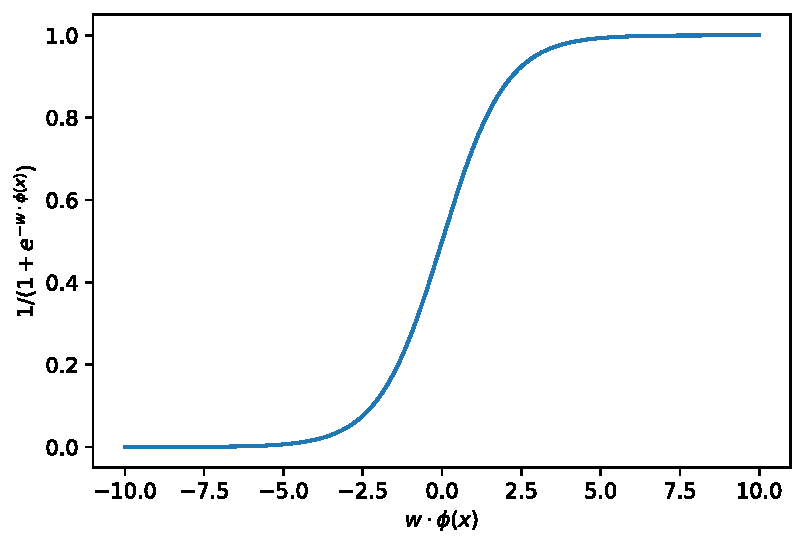
\includegraphics[height=4cm]{figures/logistic}
    \end{center}
    \vspace{-2em}
    \begin{align*}
    p(y=1\mid x; w) &= \frac{1}{1 + e^{-w\cdot\phi(x)}} \quad (y\in \pc{0,1})\\
        p(y=k\mid x; w) &= \frac{e^{w_k\cdot\phi(x)}}{\sum_{i\in\mathcal{Y}}e^{w_i\cdot\phi(x)}} \quad (y\in \pc{1, \ldots, K}) && \text{``softmax''}
    \end{align*}
    \pdfnote{
        Note that in multiclass classification setting, there is one $w$ for each class.
    }
\end{frame}

\begin{frame}
    {Inference}
    \begin{align}
        \hat{y} &= \argmax_{k\in\sY} p(y=k\mid x; w) \\
        &= \argmax_{k\in\sY} \frac{e^{w_k\cdot\phi(x)}}{\sum_{i\in\mathcal{Y}}e^{w_i\cdot\phi(x)}} \\
        &= \argmax_{k\in\sY} e^{w_k\cdot\phi(x)} \\
        &= \argmax_{k\in\sY} \underbrace{w_k\cdot\phi(x)}_{\textstyle\text{score for class $k$}}
    \end{align}
\end{frame}

\begin{frame}
    {MLE for logistic regression}
    $$
    \max \sum_{i=1}^n \log p(y^{(i)}\mid x^{(i)}; w) 
    $$
    \begin{itemize}
        \item Likelihood function is concave / NLL is convex
            \pause
        \item No closed-form solution 
        \item Use stochastic gradient ascent 
    \end{itemize}
    \pdfnote{LR is probabilistic, so we can still do MLE.}
    \pdfnote{Is there a closed form solution?}
\end{frame}

\begin{frame}
    {BoW representation}
    Example:
    \begin{align*}
        \mathcal{V} &= \pc{\w{the}, \w{a}, \w{an}, \w{in}, \w{for}, \w{penny}, \w{pound}}\\
        \text{sentence} &= \w{in for a penny, in for a pound} \\
        x &= \p{\w{in}, \w{for}, \w{a}, \w{penny}, \w{in}, \w{for}, \w{a}, \w{pound}}
    \end{align*}

    \textbf{Feature extractor}: $\phi\colon \mathcal{V}^n \rightarrow \mathbb{R}^d$.
    \pause

    \textbf{Idea}: a sentence is the ``sum'' of words.
    $$
    \phi_{\text{BoW}}(x) = \sum_{i=1}^n \phi_{\text{one-hot}}(x_i)
    $$
    \vspace{-1em}

    \begin{align*}
        \phi_{\text{one-hot}}(x_1) &= \begin{bmatrix} 0 & 0 & 0 & 1 & 0 & 0 & 0 \end{bmatrix}
        \quad \text{the sentence contains the word ``in''}\\
        \phi_{\text{BoW}}(x)  &= \begin{bmatrix} 0 & 2 & 0 & 2 & 2 & 1 & 1 \end{bmatrix}
        \quad \text{the sentence contains 2 occurrences of ``in''}\\
    \end{align*}
\end{frame}

%\begin{frame}
%    {Compare with naive Bayes}
%    \begin{itemize}
%        \itemsep2em
%        \item Our naive Bayes model ($x_i \in \pc{1, \ldots, |\sV|}$):
%            $$
%            X_i \mid Y=y \sim \text{Categorical}(\theta_{1,y}, \ldots, \theta_{|\sV|, y}) \;.
%            $$
%        \item The naive Bayes generative story produces a BoW vector following a multinomial distribution:
%            $$
%            \phi_{\text{BoW}}(X) \mid Y=y \sim \text{Multinomial}(\theta_{1,y}, \ldots, \theta_{|\sV|,y}, n) \;.
%            $$
%
%        \pause
%        \item Both multinomial naive Bayes and logistic regression learn a linear separator $w\cdot\phi_{\text{BoW}}(x)+b=0$.
%    \end{itemize}
%    \pause
%    Question: what's the advantage of using logistic regression?
%
%    \pdfnote{
%        In this sense, NB is trying to model the BoW feature vector.
%    }
%    \pdfnote{
%        In addition, they both learn a linear predictor which simply sums the score of each word at inference time.
%        For NB, $w$ is $\log \theta$.
%    }
%\end{frame}

%\begin{frame}
%    {Feature vectors for multiclass classification}
%    Multinomial logistic regression
%    \begin{tikzpicture}
%        \node (a) {
%            \begin{minipage}{\textwidth}
%            \begin{align*}
%        p(y=k\mid x; w) =
%             \frac{e^{{\color{blue}w_k\cdot\phi(x)}}}
%                {\sum_{i\in\mathcal{Y}}e^{w_i\cdot\phi(x)}} \quad (y\in \pc{1, \ldots, K})
%            \end{align*}
%            \end{minipage}
%};
%        \node(b) [below= of a] {
%            \begin{minipage}{\textwidth}
%    $$
%        p(y=k\mid x; w) =
%                \frac{e^{{\color{blue}w\cdot\Psi(x, k)}}}{\sum_{i\in\mathcal{Y}}e^{w\cdot\Psi(x, i)}} \quad (y\in \pc{1, \ldots, K})
%    $$
%            \end{minipage}
%};
%        \draw[arrow] (a) -- (b);
%    \end{tikzpicture}
%    scores of each class $\rightarrow$ compatibility of an input and a label
%
%    \pause
%    Multivector construction of $\Psi(x,y)$:
%    $$
%    \Psi(x, 1) \eqdef \pb{\underbrace{0}_{\textstyle y=0}, \underbrace{\phi(x)}_{\textstyle y=1}, \ldots, \underbrace{0}_{\textstyle y=K}}
%    $$
%\end{frame}

\begin{frame}
    {N-gram features}
    Potential problems with the the BoW representation?

    \pause
    \textbf{N-gram} features:
    \begin{center}
        \textit{in for a penny , in for a pound}
    \end{center}
    \begin{itemize}
        \item Unigram: in, for, a, ...
        \item Bigram: in/for, for/a, a/penny, ...
        \item Trigram: in/for/a, for/a/penny, ...
    \end{itemize}

    \think{What are the pros/cons of using higher order n-grams?}
    \pdfnote{
        BoW problem: new york, don't like
    }
\end{frame}

\begin{frame}
    {Feature extractor}
    Logistic regression allows for richer features (what's the limitation of NB?)

    Define each feature as a function $\phi_i\colon \mathcal{X} \rightarrow \BR$.
    \begin{align*}
 \phi_1(x) &= \begin{cases}
 1 & \text{$x$ contains ``happy''} \\
 0 & \text{otherwise}
 \end{cases} ,
 \\
 \phi_2(x) &= \begin{cases}
 1 & \text{$x$ contains words with suffix ``yyyy''} \\
 0 & \text{otherwise}
 \end{cases} .
    \end{align*}
    In practice, use a dictionary
    $$
    \texttt{feature\_vector}[\texttt{"prefix=un+suffix=ing"}] = 1
    $$
    \pdfnote{
        With NB, we can still include these features as variables, but we'll have to think about modeling them as a parametrized distribution and handling the sparsity problem during estimation.
    }
\end{frame}


%\section{Regularization, model selection, evaluation}
%
%\begin{frame}
%    {Error decomposition}
%    Let's ignore the optimization error, assuming we always find the optimum
%$$
%        \text{risk}(\hat{h}) - \text{risk}(h^*) = \text{approximation error} + \text{estimation error}
%        $$
%        \vspace{-3em}
%    \begin{itemize}
%        \itemsep1em
%        \item Approximation error:
%            $\text{risk}(\text{best hypo in $\sH$}) - \text{risk}(h^*)$ \\
%            Does my hypothesis space contain the true hypothesis?
%        \item Estimation error:
%            $\text{risk}(\hat{h}) - \text{risk}(\text{best hypo in $\sH$})$ \\
%            Can I find the best hypothesis given limited data?
%    \end{itemize}
%
%    \pause
%    Larger hypothesis class: approximation error $\downarrow$, estimation error $\uparrow$
%
%    Smaller hypothesis class: approximation error $\uparrow$, estimation error $\downarrow$
%
%    How to control the size of the hypothesis class?
%\end{frame}
%
%\begin{frame}
%    {Reduce the dimensionality}
%    Linear predictors: $\sH = \pc{w : w \in \BR^d}$
%
%    Reduce the number of features. (Ideas for text classification?)
%    \pdfnote{
%        stopwords, stemming, filter by frequency
%    }
%    \pdfnote{
%        feature selection (fwd/bwd), L1
%    }
%
%    \pause
%    For other predictors:\\
%    \begin{itemize}
%        \item Depth of decision trees
%        \item Degree of polynomials
%        \item Number of decision stumps in boosting
%    \end{itemize}
%\end{frame}
%
%\begin{frame}
%    {Regularization}
%    Reduce the ``size'' of $w$:
%    $$
%    \min_w \underbrace{\frac{1}{N}\sum_{i=1}^N L(x^{(i)}, y^{(i)}, w)}_{\textstyle \text{average loss}}
%    + \underbrace{\frac{\lambda}{2}\|w\|_2^2}_{\textstyle \ell_2 \text{ norm}}
%    $$
%
%    Why is small norm good? Small change in the input doesn't cause large change in the output.
%
%\end{frame}
%
%\begin{frame}
%    {Gradient descent with $\ell_2$ regularization}
%    Run SGD on 
%    $$
%    \min_w \underbrace{\frac{1}{N}\sum_{i=1}^N L(x^{(i)}, y^{(i)}, w)}_{\text{average loss}}
%    + \underbrace{\frac{\lambda}{2}\|w\|_2^2}_{\ell_2 \text{ norm}}
%    $$
%
%    Also called \textbf{weight decay} in the deep learning literature:
%    $$
%    w \leftarrow w - \eta(\nabla_w L(x, y, w) + {\color{blue}\lambda w})
%    $$
%
%    Shrink $w$ in each update.
%\end{frame}
%
%\begin{frame}
%    {Hyperparameter tuning}
%    \textbf{Hyperparameters}: parameters of the learning algorithm (not the model)
%
%    Example: use MLE to learn a logistic regression model using BoW features \\
%    \bigskip
%    \pause
%
%    \pause
%    How do we select hyperparameters?\\
%    \begin{itemize}
%        \item[] Pick those minimizing the training error?
%        \item[] Pick those minimizing the test error?
%    \end{itemize}
%    \pdfnote{What are the hyperparams in this case?}
%    \pdfnote{
%        Dillema: training error overfit. test error don't know.
%    }
%\end{frame}
%
%\begin{frame}
%    {Validation}
%    \textbf{Validation set}: a subset of the training data reserved for tuning the learning algorithm (also called the \textbf{development set}).
%
%    \textbf{$K$-fold cross validation}\\
%    {[board]}
%
%    \pause
%    It's important to look at the data and errors during development, but \textcolor{red}{not the test set}.
%\end{frame}
\end{document}
